\documentclass{beamer}

\usepackage{listings}
\usepackage{amsmath}
\usepackage{amsfonts}
\usepackage{amssymb}
\usefonttheme{serif}

\usepackage{MnSymbol,wasysym}

\usepackage[backend=bibtex,citestyle=authoryear]{biblatex}
\addbibresource{smoothing_rBergomi}
%\bibliography{} 


%\usepackage{multibox,fancybox}
\usepackage{epsfig}
\usepackage{graphicx,color}
\usepackage{subcaption}
\captionsetup{compatibility=false}
\usepackage{epstopdf}

\usepackage{beamerthemesplit}
\usepackage[belowskip=-15pt,aboveskip=0pt]{caption}
\usepackage{booktabs}
\usepackage{multirow}
\setbeamercovered{highly dynamic}
\usepackage{oubraces}
%\usepackage[UglyObsolete,tight,heads=LaTeX] {diagrams}
\usepackage{pifont}
\usepackage{tikz}

\usepackage{hyperref}


\usepackage{lastpage}

\newcounter{sauvegardeenumi}
\newcommand{\asuivre}{\setcounter{sauvegardeenumi}{\theenumi}}
\newcommand{\suite}{\setcounter{enumi}{\thesauvegardeenumi}}


\newcounter{saveenumi}
\newcommand{\seti}{\setcounter{saveenumi}{\value{enumi}}}
\newcommand{\conti}{\setcounter{enumi}{\value{saveenumi}}}



\addtobeamertemplate{navigation symbols}{}{%
	\usebeamerfont{footline}%
	\usebeamercolor[fg]{footline}%
	\hspace{1em}%
	\insertframenumber
}



\renewcommand{\inserttotalframenumber}{\pageref{lastslide}}

%\setbeamertemplate{caption}[numbered]
\numberwithin{figure}{section}



\graphicspath{{Figures/}{/}}
%\theoremstyle{plain}
%\newtheorem{defn}{Definition}
%\newtheorem*{claim}{Claim}



%\useoutertheme{sidebar}
%\useoutertheme{miniframes}

%
\usetheme{Boadilla}


\setbeamertemplate{caption}{\insertcaption}

%\usefonttheme{Serif}

%\usecolortheme{lily}

%\useoutertheme{infolines}

% Commands



\definecolor{cec1d24}{RGB}{236,29,36}
\definecolor{cffffff}{RGB}{255,255,255}

\newcommand{\cmark}{\ding{51}}
\newcommand{\ucmark}{\tikz[y=0.80pt,x=0.80pt,yscale=-0.02,xscale=0.02, inner sep=0pt, outer sep=0pt]%
  {\path[fill=cec1d24,nonzero rule] (635.8833,600.0000) .. controls
    (651.0771,599.6647) and (665.7558,591.6224) .. (673.9783,577.5525) .. controls
    (682.1001,563.3625) and (681.7384,546.6500) .. (674.5074,533.1862) --
    (378.4699,21.6487) .. controls (370.6590,8.7662) and (356.3424,0.0975) ..
    (340.1099,-0.0063) .. controls (323.6499,0.0972) and (309.3362,8.7657) ..
    (301.4862,21.6487) -- (5.4612,533.1862) .. controls (-1.7257,546.6500) and
    (-2.0877,563.3625) .. (5.9903,577.5525) .. controls (14.2570,591.6225) and
    (28.9353,599.6650) .. (44.0853,600.0000) -- (635.8853,600.0000);
    \path[fill=cffffff,nonzero rule] (340.1208,75.7875) -- (71.0683,540.8450) --
    (608.8933,540.8450) -- (340.1058,75.7950);
    \path[fill=black,nonzero rule] (303.5900,225.7800) .. controls
    (280.4500,225.7300) and (276.9200,248.1400) .. (276.8800,250.6200) .. controls
    (276.9200,262.4400) and (285.4000,277.1700) .. (309.1600,279.4100) .. controls
    (309.1600,279.4100) and (313.7700,280.0900) .. (313.6600,283.0900) .. controls
    (313.7700,285.9400) and (313.7800,284.9700) .. (312.3400,286.5300) .. controls
    (310.8500,288.2300) and (298.5500,299.6400) .. (298.3100,302.6600) .. controls
    (296.9800,316.8800) and (300.1800,335.2800) .. (303.0900,345.9400) .. controls
    (303.0900,345.9400) and (306.6000,354.7800) .. (303.8800,361.0000) .. controls
    (301.0600,367.4700) and (289.0000,397.7400) .. (288.0000,399.5600) .. controls
    (285.1300,404.8200) and (284.0000,409.1400) .. (285.8800,415.4100) .. controls
    (284.6600,416.1100) and (264.4700,428.8800) .. (264.4700,428.8800) .. controls
    (264.4700,428.8800) and (261.3500,421.5100) .. (253.5900,419.3800) .. controls
    (245.7000,417.1100) and (239.1800,418.1800) .. (232.7200,405.9100) --
    (226.8800,396.4100) .. controls (226.8800,396.4100) and (225.6700,392.9300) ..
    (219.7500,391.6200) .. controls (213.9300,390.4900) and (206.1000,388.3000) ..
    (202.8100,388.4700) .. controls (198.6100,388.8800) and (195.2200,387.7300) ..
    (189.5900,394.2800) .. controls (185.0800,399.5300) and (112.8800,524.4700) ..
    (112.8800,524.4700) -- (286.4100,524.4700) .. controls (286.4100,524.4700) and
    (290.7100,524.0000) .. (289.5900,519.9700) .. controls (288.2700,516.1900) and
    (267.3800,441.8100) .. (267.3800,441.8100) -- (291.4400,426.7500) .. controls
    (291.4400,426.7500) and (293.3600,429.9900) .. (300.4400,426.7500) .. controls
    (307.3800,423.4800) and (309.9700,421.7500) .. (309.9700,421.7500) .. controls
    (309.9700,421.7500) and (313.9200,421.4900) .. (313.4100,413.0300) .. controls
    (316.1700,411.3100) and (341.9700,395.0600) .. (341.9700,395.0600) .. controls
    (341.9700,395.0600) and (332.8400,417.6000) .. (331.9100,427.5600) .. controls
    (331.2100,437.4600) and (327.6900,504.1200) .. (327.6900,504.1200) .. controls
    (327.6900,504.1200) and (328.1300,509.2200) .. (324.7800,510.2200) .. controls
    (321.2800,511.1700) and (305.7200,515.5000) .. (305.7200,515.5000) .. controls
    (305.7200,515.5000) and (301.3900,516.2100) .. (301.5000,519.7200) .. controls
    (301.3900,523.0400) and (303.0200,524.3400) .. (304.9400,524.4700) .. controls
    (306.9300,524.3400) and (355.7200,524.4700) .. (355.7200,524.4700) .. controls
    (355.7200,524.4700) and (360.7100,525.0000) .. (361.5300,518.4100) .. controls
    (362.3400,511.9900) and (371.5900,445.5000) .. (371.5900,445.5000) .. controls
    (371.5900,445.5000) and (367.5700,444.4500) .. (367.6200,440.5000) .. controls
    (367.5700,436.3200) and (367.5600,433.2000) .. (368.9400,431.5000) .. controls
    (370.1600,429.9500) and (384.8300,413.0400) .. (394.8800,389.5300) .. controls
    (396.4200,386.0300) and (397.5600,389.1300) .. (397.7800,390.0600) .. controls
    (398.2100,390.7500) and (417.2800,442.6600) .. (419.4700,444.7200) .. controls
    (421.8400,446.5600) and (473.3600,488.2300) .. (474.5000,489.0900) .. controls
    (475.6400,489.8600) and (478.9100,492.1100) .. (479.0000,499.3800) .. controls
    (478.9100,506.7600) and (475.9700,512.6300) .. (473.9700,514.9700) .. controls
    (472.0500,517.1900) and (468.8000,520.4500) .. (468.6900,521.8400) .. controls
    (468.8000,523.3800) and (470.2800,524.3400) .. (471.3400,524.4700) .. controls
    (472.5600,524.3400) and (479.2500,524.3400) .. (479.8100,524.4700) .. controls
    (480.5500,524.3400) and (489.3400,525.0100) .. (495.4100,514.1900) .. controls
    (501.7300,503.5300) and (513.1200,484.3400) .. (513.1200,484.3400) .. controls
    (513.1200,484.3400) and (515.5800,480.5600) .. (512.0600,478.2500) .. controls
    (508.4000,476.0100) and (502.7100,474.7100) .. (499.3800,471.1200) .. controls
    (495.8600,467.5500) and (462.9400,429.6400) .. (462.3400,428.8800) .. controls
    (461.9600,428.3400) and (457.7100,423.7600) .. (452.2800,426.2200) .. controls
    (450.7000,424.0900) and (448.8400,421.2200) .. (448.8400,421.2200) .. controls
    (448.8400,421.2200) and (439.4600,364.4600) .. (429.5300,340.4100) .. controls
    (431.8000,339.0000) and (434.8100,336.7200) .. (434.8100,336.7200) .. controls
    (434.8100,336.7200) and (442.7200,343.5500) .. (449.3800,336.4400) .. controls
    (456.0900,329.2300) and (455.6000,329.4100) .. (454.4100,326.1600) .. controls
    (453.3200,322.9000) and (452.8300,321.9100) .. (450.4400,320.5900) .. controls
    (448.2700,319.3000) and (444.5200,315.5500) .. (444.6200,308.9700) .. controls
    (444.5200,302.5400) and (441.7400,284.8000) .. (438.5300,277.2800) .. controls
    (435.5500,269.8300) and (434.5600,261.5500) .. (422.9100,256.4400) .. controls
    (404.4800,248.2100) and (379.8000,243.3100) .. (361.8100,247.9700) .. controls
    (356.8300,249.3000) and (340.8200,261.0500) .. (339.3100,261.9700) .. controls
    (337.8900,262.6800) and (331.6400,265.2600) .. (332.1900,259.8400) .. controls
    (333.4500,247.4700) and (322.7500,225.7300) .. (303.5900,225.7800) --
    cycle(394.8800,275.9700) .. controls (394.8800,275.9700) and
    (408.4700,275.8400) .. (411.5300,276.2200) .. controls (414.3400,276.5000) and
    (416.0300,280.1900) .. (416.0300,280.1900) -- (429.0000,325.8800) --
    (424.2500,328.7800) .. controls (421.5800,323.2700) and (397.9000,287.2600) ..
    (393.0300,280.4700) .. controls (389.9100,276.1000) and (394.8800,275.9700) ..
    (394.8800,275.9700) -- cycle(331.0000,332.8100) .. controls
    (331.5700,332.7900) and (332.2200,332.9700) .. (332.7200,333.2800) .. controls
    (337.8300,336.2000) and (347.5100,344.5400) .. (355.7200,356.0000) .. controls
    (356.7000,357.3200) and (355.7200,361.2800) .. (355.7200,361.2800) --
    (348.5900,376.0600) .. controls (348.5900,376.0600) and (317.8500,395.3700) ..
    (315.5000,396.9100) .. controls (312.9600,398.3000) and (311.5500,396.9300) ..
    (313.9400,393.7500) .. controls (327.6400,375.1200) and (332.7200,353.0000) ..
    (329.5300,335.1200) .. controls (329.2600,333.4800) and (330.0500,332.8500) ..
    (331.0000,332.8100) -- cycle;}}
\newcommand{\ceil}[1]{\lceil {#1} \rceil}
\newcommand{\seqof}[3]{(#1)_{#2}^{#3}}

\newcommand{\ssa}{\text{SSA}}
\newcommand{\hyb}{\text{Hyb}}
\newcommand{\MNRM}{\text{MNRM}}
\newcommand{\TL}{\text{TL}}
\newcommand{\ML}{\text{ML}}
\newcommand{\Li}{L^{\text{int}}}
\newcommand{\Ls}{L_c^{\text{exp}}}
\newcommand{\Lc}{L_c^{\text{imp}}}


%\newcommand{\NSSA}{N_{\ssa}}
\newcommand{\NSSAKone}{N_{\ssa,K1}}
\newcommand{\NSSAKtwo}{N_{\ssa,K1'}}

%\newcommand{\NMNRMKone}{N_{\MNRM,K1}}
%\newcommand{\NMNRMKtwo}{N_{\MNRM,K2}}
%\newcommand{\NMNRMKoneC}{N_{\MNRM,K1}^{(c)}}
%\newcommand{\NMNRMKtwoC}{N_{\MNRM,K2}^{(c)}}

\newcommand{\NMNRMKone}{N_{K1}}
\newcommand{\NMNRMKtwo}{N_{K2}}
\newcommand{\NMNRMKoneC}{N_{K1}^{(c)}}
\newcommand{\NMNRMKtwoC}{N_{K2}^{(c)}}

\newcommand{\NMNRM}{N_{\MNRM}}
\newcommand{\NMNRMC}{N_{\MNRM}^{(c)}}
%\newcommand{\NMNRMP}{N_{{\MNRM}^*}}

\newcommand{\NSSAP}{N_{{\ssa}^*}}
\newcommand{\NTL}{N_{\TL}}
\newcommand{\NTLP}{N_{{\TL}^*}}
\newcommand{\NTLC}{N_{\TL}^{(c)}}
%\newcommand{\NTLF}{\dbar N_{\TL}}

\newcommand{\EE}{\mathcal{E}}

\newcommand{\WE}{\EE_I}
\newcommand{\WEC}[1]{\EE_{I,#1}}
\newcommand{\WEH}[1]{\hat \EE_{I,#1}}
\newcommand{\WSSA}{\text{Cost}_{\ssa}}
\newcommand{\WHYB}{\text{Cost}_{\hyb}}


\newcommand{\avg}[2]{\mathcal{A}\left(#1;#2\right)}
%\newcommand{\SD}[2]{\mathcal{S}(#1;#2)}
\newcommand{\svar}[2]{\mathcal{S}^2\left(#1;#2\right)}

\newcommand{\dbar}[1]{\Bar{\Bar{#1}}}

\newcommand{\ie}{\emph{i.e.}}
\newcommand{\eg}{\emph{e.g.}}
\newcommand{\cf}{\emph{cf.}}
\newcommand{\ud}{\mathrm{d}}
\newcommand{\prob}[1]{\mathrm{P}\left(#1\right)}
\newcommand{\expt}[1]{\mathrm{E}\left[#1\right]}
\newcommand{\expth}[1]{\hat{\mathrm{E}}\left[#1\right]}

\newcommand{\var}[1]{\mathrm{Var}\left[#1\right]}
\newcommand{\cov}[2]{\mathrm{Cov}\left[#1, #2\right]}
\newcommand{\norm}[1]{\left\|#1\right\|}
\newcommand{\abs}[1]{\left|#1\right|}
\newcommand{\rset}{\mathbb{R}}
\newcommand{\nset}{\mathbb{N}}
\newcommand{\zset}{\mathbb{Z}}
\newcommand{\JAC}{\mathbb{J}}
\newcommand{\one}{\mathbf{1}}
\newcommand{\poisson}[1]{\mathcal{P}\left(#1\right)}
\newcommand{\normal}[1]{\mathcal{N}\left(#1\right)}
\newcommand{\binomial}[1]{\mathcal{B}\left(#1\right)}
\newcommand{\Ordo}[1]{{\mathcal{O}}\left(#1\right)}
\newcommand{\OrdoP}[1]{{\mathcal{O}_P}\left(#1\right)}
\newcommand{\ordo}[1]{{o}\left(#1\right)}
\newcommand{\abstr}[1]{\begin{abstract}#1\end{abstract}}
\newcommand{\thx}[1]{\thanks{#1}}
\newcommand{\red}[1]{{\color{red}#1}}
\newcommand{\blue}[1]{{\color{blue}#1}}
\newcommand{\green}[1]{{\color{magenta}#1}}

\newcommand{\latt}{\mbox{$\zset_+^d$}}


%Alvaro's notations

\newcommand{\indicator}[1]{\mathbf{1}_{#1}} 

\newcommand{\PERIOD}{.}
\newcommand{\COMMA}{,}

% Removed this command since it does not work properly with spacing
%\newcommand{\ChB}{{Chernoff bound }}
\newcommand{\LP}{\left(}
\newcommand{\RP}{\right)}

\newcommand{\LPe}{\left.}
\newcommand{\RPe}{\right.}

%\newcommand{\SEP}{\biggm|}
\newcommand{\SEP}{\, \big| \,}
\newcommand{\BX}{\bar X(t)}
\newcommand{\BXi}{\bar X_i(t)}
\newcommand{\BXitau}{\bar X_i(t{+}\tau)}

\newcommand{\sj}{\sum_{j=1}^J}

\newcommand{\Qi}{Q_i(t,\tau_i)}
\newcommand{\lji}{a_j(\bar X(t))\tau_i}
\newcommand{\Yj}{Y_j\left( a_j(\bar X(t))\tau_i \right)}
\newcommand{\ldi}{\log(\delta_i)}
\newcommand{\taui}{\tau_i(s)}
\newcommand{\DEN}[1]{- a_0 \LP \bar X(t) \RP +  \sj a_j(\bar X(t))e^{-#1\, \nu_{ji}}}
\newcommand{\aj}{ a_j(\bar X(t))}

\newcommand{\anu}{\sj \aj \nu_{ji}}
%\newcommand{\anu2}{\sj \aj (\nu_{ji})^2}
\newcommand{\tsi}{\tilde{s}_i}
\newcommand{\hs}{\hat{s}}
%\newcommand{\tti1}{\tilde{t}_{i,1}} 
\newcommand{\az}{a_0(\bar X(t))}
\newcommand{\dnux}{\delta_i^{\,\nu_{ji}/{\BXi}}}

\newcommand{\bj}{b_{ji}(\bar X(t))}
\newcommand{\mE}[1]{\mathcal{E}_{#1}}
\newcommand{\mV}[1]{\mathcal{V}_{#1}}
\newcommand{\hmV}[1]{\hat{\mathcal{V}}_{#1}}

\newcommand{\orden}{\alpha}

%Pedro's notations
\newcommand{\X}[1]{\bar X(t_{#1})}
\newcommand{\ti}[1]{t_{#1}}
%\newcommand{\iff}{\Leftrightarrow}

\newcommand{\algorithmfootnote}[2][\footnotesize]{%
  \let\old@algocf@finish\@algocf@finish% Store algorithm finish macro
  \def\@algocf@finish{\old@algocf@finish% Update finish macro to insert "footnote"
    \leavevmode\rlap{\begin{minipage}{\linewidth}
    #1#2
    \end{minipage}}%
  }%
}
%new command for switch case algo
% New definitions
%\algnewcommand\algorithmicswitch{\textbf{switch}}
%\algnewcommand\algorithmiccase{\textbf{case}}
%\algnewcommand\algorithmicassert{\texttt{assert}}
%\algnewcommand\Assert[1]{\State \algorithmicassert(#1)}%
%
%% New "environments"
%\algdef{SE}[SWITCH]{Switch}{EndSwitch}[1]{\algorithmicswitch\ #1\ \algorithmicdo}{\algorithmicend\ \algorithmicswitch}%
%\algdef{SE}[CASE]{Case}{EndCase}[1]{\algorithmiccase\ #1}{\algorithmicend\ \algorithmiccase}%
%\algtext*{EndSwitch}%
%\algtext*{EndCase}%

%%% Local Variables: 
%%% mode: latex
%%% TeX-master: "main_new"
%%% End: 




%\author[Outline]{Chiheb BEN HAMMOUDA (KAUST, Saudi Arabia)
% Alvaro Moraes (KAUST, Saudi Arabia)
% Ra\'ul Tempone (KAUST, Saudi Arabia)}

\institute{\scalebox{1.5}{\insertlogo}}
\setbeamercolor{author in head/foot}{bg=black,fg=white}
\setbeamertemplate{caption}[numbered]

% footline all over the presentation
\setbeamertemplate{footline}
{
	\leavevmode
	\hspace{-0.25cm}
	\hbox{
		\begin{beamercolorbox}[wd=.2\paperwidth,ht=0.4cm,dp=1.125ex,center]{author in head/foot}%
			\usebeamerfont{title in head/foot}
			\vspace{0.05cm} Chiheb Ben Hammouda, Alvaro Moraes and Raul Tempone
			\vspace{0.05cm}
			Computer, Electrical and Mathematical Science \& Engineering Division\\ King Abdullah University of Science and Technology (KAUST), Saudi Arabia
			\hspace{.3cm}
		\end{beamercolorbox}%
		
		\begin{beamercolorbox}[wd=.6\paperwidth,ht=0.4cm,dp=1.125ex,center]{title in head/foot}%tive Radio Systems
			\usebeamerfont{author in head/foot}
			\center{\vspace{0.03cm}\title{Hierarchical Stochastic  Methods for  Option Pricing and Stochastic Reaction Networks}}
		\end{beamercolorbox}%
		
		\begin{beamercolorbox}[wd=.12\paperwidth,ht=0.4cm,dp=1.125ex,left]{author in head/foot}
			\usebeamerfont{title in head/foot}
			\center{April 2015}
		\end{beamercolorbox}
		
		\begin{beamercolorbox}[wd=.08\paperwidth,ht=0.4cm,dp=1.125ex,center]{title in head/foot}%
			\usebeamerfont{author in head/foot}
			\insertframenumber / \inserttotalframenumber
		\end{beamercolorbox}%
	}
}


\setbeamertemplate{headline}
{%
	\leavevmode%
	\begin{beamercolorbox}[wd=0.5\paperwidth,ht=5ex,dp=4ex]{section in head/foot}%
		\hbox to .5\paperwidth{\hfil\insertsectionhead\hfil}
	\end{beamercolorbox}%
	\begin{beamercolorbox}[wd=0.5\paperwidth,ht=5ex,dp=4ex]{subsection in head/foot}%
		\hbox to .5\paperwidth{\hfil \insertsubsectionhead \hfil}
	\end{beamercolorbox}%
}
\renewcommand*{\inserttotalframenumber}{\pageref{lastframe}}
%%%%%%%%%%%%%%%%%%%%%%%%%%%%%%%%%%%%%%%%%%%%%%%%%%%%%%%%%%%%%%%%%%%%%%%%%%%%%%%%%%%%%%%%%%%%%%%%%%%%%%%%%%%%%%%%%%%%%%%%%%%%%%%%%%%%%%%%%%%%%%%%%%%%%%%%
%%%%%%%%%%%%%%%%%%%%%%%%%%%%%%%%%%%%%%%%%%%%%%%%%%%%%%%%%%%%%%%%%%%%%%%%%%%%%%%%%%%%%%%%%%%%%%%%%%%%%%%%%%%%%%%%%%%%%%%%%%%%%%%%%%%%%%%%%%%%%%%%%%%%%%%%%%
%%%%%%%%%%%%%%%%%%%%%%%%%%%%%%%%%%%%%%%%%%%%%%%%%%%%%%%%%%%%%%%%%%%%%%%%%%%%%%%%%%%%%%%%%%%%%%%%%%%%%%%%%%%%%%%%%%%%%%%%%%%%%%%%%
%%%%%%%%%%%%%%%%%%%%%%

\title[Short title]{\centerline{Adaptive sparse  grids and quasi Monte Carlo  } \\
	\centerline{
			for option pricing under the rough Bergomi model }}


\author[Short Name (U ABC)]{%
  \texorpdfstring{%
    \begin{columns}
      \column{.5\linewidth}
      \centering
     Chiheb Ben Hammouda \\	\begin{figure}[!htb]
							
\includegraphics[scale=0.18]{kaust}
 							\end{figure}
    \end{columns}
    \vspace{12pt}
    \begin{columns}
      \column{.3\linewidth}
      \centering
      Christian Bayer \\    \begin{figure}[!htb]
							
\includegraphics[scale=0.2]{WIAS}
 							\end{figure}
      \column{.3\linewidth}
      \centering
     Ra\'ul Tempone	 \\ \begin{figure}[!htb]
							
\includegraphics[scale=0.25]{rwth}
 							\end{figure}
    \end{columns}
 }
 {Chiheb Ben Hammouda, Christian Bayer, Ra\'ul Tempone	}
}

\date[July  2019]{3rd International Conference on
Computational Finance (ICCF2019), A Coru\~na\\ 
					8-12 July,  2019 }

%%\setbeamertemplate{caption}[numbered]
%%\frame{\titlepage}
%
%%\begin{frame}[plain]
%%	\frametitle{\centerline{Adaptive sparse  grids and quasi Monte Carlo  } \\
%%		\centerline{
%%			for option pricing under the rough Bergomi model }}
%%	
%%	\setbeamercolor{block body}{use=structure,fg=black,bg=white!30!blue}
%	
%	
%	
%	\vspace{0.3cm}
%	\begin{center}
%		Chiheb Ben Hammouda \\
%	\end{center}
%	
%	
%	\vspace{0.2cm}
%	\begin{center}	
%	\textbf{Joint work with}: Christian Bayer  \& Ra\'ul Tempone		
%	\end{center}
%	\vspace{0.1cm}
%	\begin{center}
%		\today 
%	\end{center}
%	
%		
%	\vspace{0.2cm}
%	\begin{figure}[!htb]
%		
\includegraphics[scale=0.2]{kaust.jpg}
%	\end{figure}
%	\vspace{0.2cm}
%%\end{frame}




%------------------------------
\begin{document}
\begin{frame}[plain,noframenumbering]
  \maketitle
\end{frame}
%
%\begin{frame}[plain,noframenumbering]
%	\frametitle{\centerline{Outline}}
%	 \tableofcontents
%\end{frame}






\section{Option Pricing under the Rough Bergomi Model: Motivation \& Challenges}
\frame[plain,noframenumbering]
{\tableofcontents[currentsection,currentsubsection]}





\begin{frame}[plain]\frametitle{\centerline{Rough volatility \footnote{\fullcite{gatheral2018volatility}}}}
		\begin{figure}
		\centering
		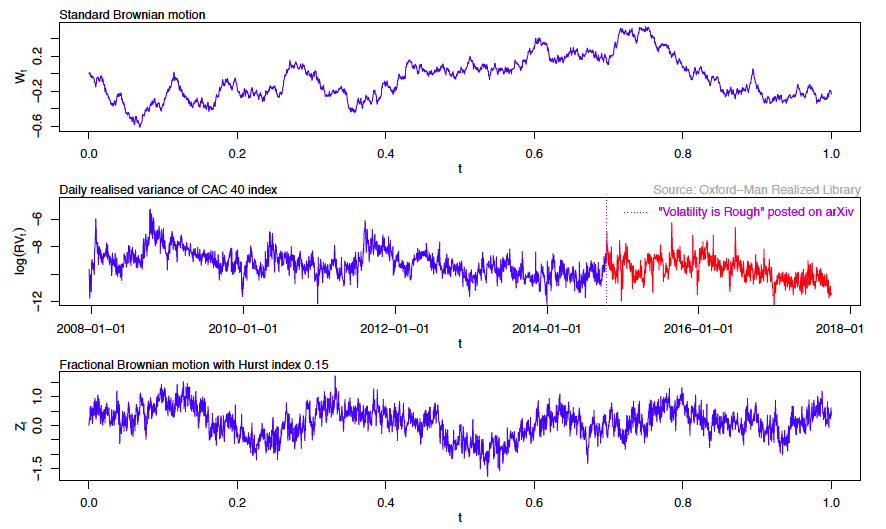
\includegraphics[scale=0.4]{vol_rough}
%		\caption{}
		\label{fig:vol_rough}
	\end{figure}
\end{frame}




\begin{frame}[plain]\frametitle{\centerline{The rough Bergomi model \footnote{\fullcite{bayer2016pricing}}}}
\vspace{0.2cm}
This model, under a pricing measure, is given by

\begin{equation}
\begin{small}
\begin{cases}
	dS_t &= \sqrt{v_t} S_t dZ_t,\\
v_t &= \blue{\xi_0}(t) \exp\left( \blue{\eta} \widetilde{W}_t^{\blue{H}} - \frac{1}{2} \blue{\eta}^2 t^{2\blue{H}} \right),\\
	Z_t&:=\blue{\rho}	W^1_t+ \bar{\rho}W^\perp_t \equiv \blue{\rho} W^1+\sqrt{1-\blue{\rho}^2} W^\perp,
\end{cases}
\end{small}
\end{equation}
\begin{itemize}
	\item $(W^1,W^\perp)$: two independent standard Brownian motions
	\item $\widetilde{W}^\blue{H} $ is \red{Riemann-Liouville process},  defined by
	\begin{align*}
	\widetilde{W}_t^{\blue{H}} &= \int_0^t K^{\blue{H}}(t-s) dW_s^1, \quad t \ge 0, \\ 	K^{\blue{H}}(t-s) &= \sqrt{2\blue{H}} (t-s)^{\blue{H} - 1/2},\quad \forall \: 0 \le s \le t.
	\end{align*}
	\item $\blue{H} \in(0,1/2]$ controls the \red{roughness} of paths,  $\blue{\rho} \in [-1,1]$  and  $\blue{\eta}>0$.
	\item $t \mapsto \blue{\xi}_0(t)$: forward variance curve, known at time $0$.
\end{itemize}
\end{frame}
\begin{frame}[plain]\frametitle{\centerline{Model challenges }}
\begin{itemize}
\item \textbf{Numerically:}
	\begin{itemize}
		\item The model is \red{non-Markovian} and   \red{non-affine} $\Rightarrow$ Standard numerical methods (PDEs, characteristic functions) seem \red{inapplicable}.
		\item The only prevalent pricing method for mere
		\red{vanilla options} is \red{Monte Carlo (MC)} \parencite{bayer2016pricing,mccrickerd2018turbocharging} \frownie{} still  \red{computationally expensive task}.
		
\item 	Discretization methods have  a \red{poor behavior of the strong error} (strong convergence rate  of order $\blue{H} \in[0,1/2]$) \parencite{neuenkirch2016order} $\Rightarrow$ Variance reduction methods, such as \red{multilevel Monte Carlo (MLMC)}, are inefficient for \red{very small values} of $\blue{H}$.
	\end{itemize}

\item \textbf{Theoretically:} 
\begin{itemize}
\item No proper weak error analysis done in the rough volatility
context.
\end{itemize}
\end{itemize}

\end{frame}



\begin{frame}[plain]	
	\frametitle{\centerline{Option pricing challenges }}

	 The integration problem is  \red{challenging}

	\begin{itemize}
		\item \blue{Issue $1$:}
		Time-discretization of the rough Bergomi process (large $\blue{N}$ (number of time steps))  $\Rightarrow$ \blue{$S$}  takes values in a high-dimensional space  $\Rightarrow$  \frownie{}  \red{Curse of dimensionality} when using numerical integration methods. 
 
		\item \blue{Issue $2$:} The payoff function \blue{$g$} is typically \red{not smooth} $\Rightarrow$ \red{low regularity}$\Rightarrow$  \frownie{}   slow convergence of deterministic quadrature methods.
	\end{itemize}
{\fontencoding{U}\fontfamily{futs}\selectfont\char 66\relax} \red{Curse of dimensionality:} An exponential growth of the work (number of function evaluations) in terms of the
dimension of the integration problem. 


\end{frame}



\begin{frame}[plain]\frametitle{\centerline{Methodology \footnote{\fullcite{bayer2018hierarchical}}}}

 We design  \red{efficient hierarchical  pricing methods} based on
		\begin{enumerate}
			\item \red{Analytic smoothing}  to uncover available regularity (inspired by \parencite{romano1997contingent} in the context of stochastic volatility models).
			\item Approximating the option price using  \red{deterministic quadrature  methods} 
			\begin{itemize}
			\item \textbf{Adaptive sparse grids quadrature (ASGQ)}.
			\item \textbf{Quasi Monte Carlo (QMC)}.
			\end{itemize}			  
			\item Coupling our methods with \red{hierarchical representations}
			\begin{itemize}
			\item \textbf{Brownian bridges} as a Wiener path generation method  $\Rightarrow$  \red{ $\searrow$ the effective dimension} of the problem.
			\item \textbf{Richardson Extrapolation} (\red{Condition: weak error of order $1$)} 
		$\quad\Rightarrow$ Faster convergence of the weak error  $\Rightarrow $ $\searrow$ number of time steps \red{(smaller dimension)}.
		\end{itemize}
		\end{enumerate} 
	
\end{frame}		
	

\begin{frame}[plain]\frametitle{\centerline{Simulation of the rough Bergomi dynamics}}
\textbf{\blue{Goal:}} Simulate jointly $(W_t^1, \widetilde{W}^H_t: 0 \le t \le T)$, resulting in $W^1_{t_1},\dots, W_{t_N}$ and $\widetilde{W}^H_{t_1},\dots, \widetilde{W}^H_{t_N}$ along a given grid $t_1 <\dots < t_N$ 
\begin{enumerate}
	
	\item  \textbf{Covariance based approach} \parencite{bayer2016pricing}
	\begin{itemize}
	\item  Based on Cholesky decomposition of the covariance matrix  of the ($2N$)-dimensional Gaussian random vector  $W^1_{t_1},\dots, W^1_{t_N}, \widetilde{W}^H_{t_1},\dots, \widetilde{W}_{t_N}$.
	\item  \red{Exact method  but slow} 
	\item At least \red{$\Ordo{N^2}$}.
\end{itemize}	
	\item  \textbf{The hybrid scheme} \parencite{bennedsen2017hybrid} 
	\begin{itemize}
	\item Based on  \red{Euler discretization}  but crucially \red{improved by moment matching} for the singular term in the left point rule.
	\item  \red{Accurate scheme that is much faster} than the  Covariance based approach.
	\item \red{$\Ordo{N}$} up to logarithmic factors that depend on the desired error.
\end{itemize}	
	\end{enumerate}
\end{frame}



\begin{frame}[plain]\frametitle{\centerline{On the choice of the simulation scheme}}
\begin{figure}[h!]
\caption{The convergence of the weak error $\mathcal{E}_B$, using MC with $6 \times 10^6$ samples, for example parameters: \red{$H=0.07,\: K=1,S_0=1,\: T=1,\: \rho=-0.9,$} \red{$\eta=1.9,\: \xi_0=0.0552$}. The upper and lower bounds are $95\%$ confidence intervals. a) With \red{the hybrid scheme}  b) With \red{the exact scheme}.}
	\centering
	\begin{subfigure}{.52\textwidth}
		\centering
		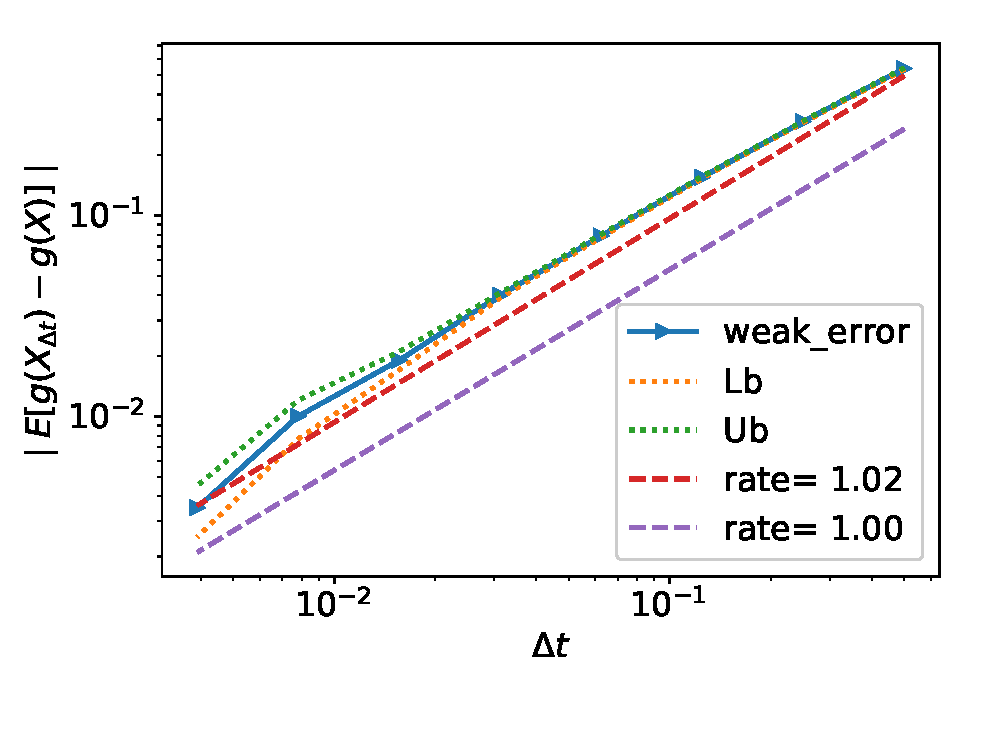
\includegraphics[width=1\linewidth]{./rBergomi_weak_error_rates/without_richardson/H_007/weak_convergence_order_Bergomi_H_007_K_1_M_4_10_6_CI_relative_hybrid_non_hierarchical_non_parallel_asymptotic}
		\caption{}
		\label{fig:set1_weak_rate_hybrid}
	\end{subfigure}%
	\begin{subfigure}{.52\textwidth}
		\centering
		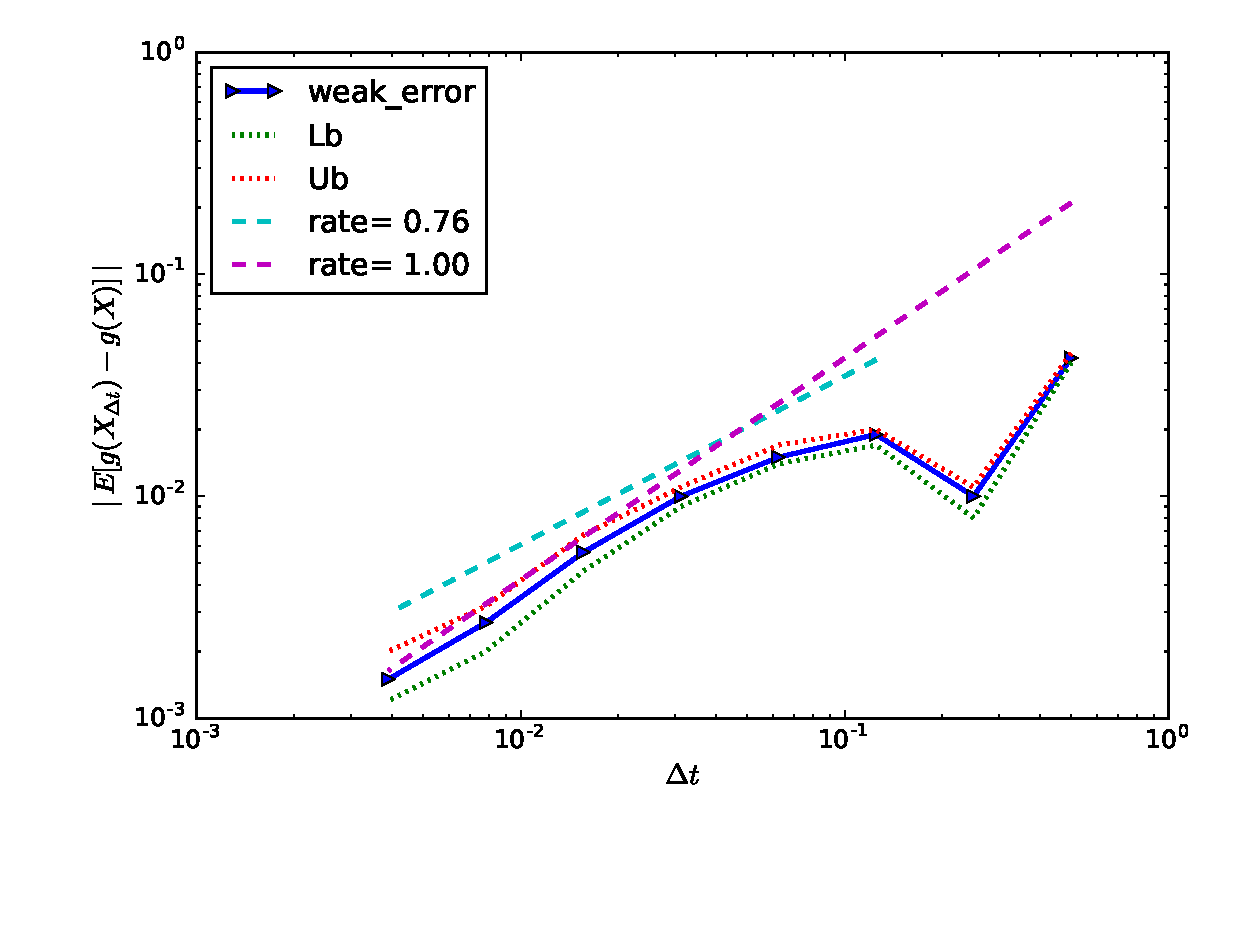
\includegraphics[width=1\linewidth]{./rBergomi_weak_error_cholesky/weak_convergence_order_Bergomi_H_007_K_1_M_4_10_6_CI_relative_cholesky_non_hierarchical_non_parallel_asymptotic}
		\caption{}
		\label{fig:set1_weak_rate_exact}
	\end{subfigure}
	\label{fig:Weak_rate_set1_set_2_without_rich_hyb+chol}
\end{figure}
\end{frame}




%\begin{frame}[plain, shrink=4]\frametitle{\centerline{Hybrid scheme \cite{bennedsen2017hybrid}}}
%\begin{small}
%\begin{align*}
%	\widetilde{W}_t^{\blue{H}} &= \int_0^t K^{\blue{H}}(t-s) dW_s^1, \quad t \ge 0, \\ 	K^{\blue{H}}(t-s) &= \sqrt{2\blue{H}} (t-s)^{\blue{H} - 1/2},\quad \forall \: 0 \le s \le t. 
%	\end{align*}
%	\end{small}
%\begin{itemize}
%\item 	The hybrid scheme \red{discretizes} the  $\widetilde{W}^\blue{H}$ process into \red{Wiener integrals of power functions and a Riemann sum}, appearing from approximating the kernel by power functions near the origin and step functions elsewhere.
%\begin{small}
%\begin{align*}
%\widetilde{W}^H_{\frac{i}{N}} \approx \overline{W}^H_{\frac{i}{N}}&= \sqrt{2H} \left(  W^2_i+\sum_{k=2}^{i} \left(\frac{b_k}{N}\right)^{H-\frac{1}{2}} \left(W_{\frac{i-(k-1)}{N}}^1-W_{\frac{i-k}{N}}^1\right)\right)\COMMA
%\end{align*}
%\end{small}
%\begin{itemize}
%\item $N$ is the number of time steps 
%\item $\{W^{2}_j\}_{j=1}^N$: \red{Artificially introduced} $N$ Gaussian random variables that are used for left-rule points in the hybrid scheme.
%\item $b_k=\left(\frac{k^{H+\frac{1}{2}}-(k-1)^{H+\frac{1}{2} }}{H+\frac{1}{2}}\right)^{\frac{1}{H-\frac{1}{2}}}.$
%\end{itemize}
%\end{itemize}
%\end{frame}
%
%



\section{Our Hierarchical Deterministic Quadrature Methods}
\frame[plain,noframenumbering]{\tableofcontents[currentsection,currentsubsection]}


\begin{frame}[plain,shrink=5]\frametitle{\centerline{Conditional expectation for analytic smoothing}}
\begin{small}
\begin{align}\label{BS_formula_rbergomi}
C_{RB}\left( T, K \right) &= E\left[ \left(S_T - K \right)^+ \right]  \nonumber\\
&=\expt{\expt{(S_T-K)^+ \mid \sigma(W^1(t) ,t \le T)}}\nonumber \\
&=E\left[C_{BS}\left( \blue{S_0} = \operatorname{exp}\left(\rho \int_0^T \sqrt{v_t} dW_t^1 - \frac{1}{2}
\rho^2 \int_0^T v_t dt\right), \right. \right.\nonumber\\
&\quad \quad \quad \left.\left.\ \blue{k} = K , \ \blue{\sigma^2} = (1-\rho^2)
\int_0^T v_t dt \right) \right]\nonumber\\
&\approx \int_{\rset^{2\red{N}}} C_{BS} \left(\blue{G}(\mathbf{w}^{(1)},\mathbf{w}^{(2)})\right) \rho_{\red{N}}(\mathbf{w}^{(1)})  \rho_{\red{N}}(\mathbf{w}^{(2)}) d\mathbf{w}^{(1)} d\mathbf{w}^{(2)}\nonumber\\
&=C_{RB}^N \PERIOD
\end{align}
\end{small}
\begin{itemize}
\item $C_{\text{BS}}(\blue{S_0},\blue{k},\blue{\sigma^2})$: the Black-Scholes call price, for initial spot price $\blue{S_0}$, strike price $\blue{k}$, and volatility $\blue{\sigma^2}$.
\item \blue{$G$} maps $2N$ independent standard Gaussian random inputs to the parameters fed to Black-Scholes formula.
\item $\rho_{\red{N}}$: the multivariate Gaussian density, $\red{N}$: number of time steps.
\end{itemize} 
\end{frame}


%\begin{frame}[plain,shrink=1]	
%	\frametitle{\centerline{ Numerical integration methods}}
%
%	\begin{itemize}
%	\item \textbf{Plain Monte Carlo (MC)}
%	\begin{itemize}
%	\item $\red{\varepsilon(M)}=\Ordo{\red{M}^{-1/2}}$ 
%	\item $(+)$ insensitive to $\blue{d}$, $(-)$ slow convergence,  no profit from regularity.
%\end{itemize}	  
%	\item \textbf{\red{Classical Quasi-Monte Carlo (QMC)}}
%	\begin{itemize}
%	\item $\red{\varepsilon(M)}=\Ordo{\red{M}^{-1}\log(\red{M})^{\blue{d}-1}}$ 
%	\item  $(+)$ better convergence, $(-)$ sensitive to $\blue{d}$, no profit from regularity.
%\end{itemize}	  
%	\item \textbf{Quadrature based on product approaches} 
%	\begin{itemize}
%	\item $\red{\varepsilon(M)}=\Ordo{\red{M}^{-\blue{r}/\blue{d}}}$
%	 \item $(+)$ profits from regularity, $(-)$ highly sensitive to $\blue{d}$.
%	\end{itemize}
%	\item \red{\textbf{Sparse grids quadrature (SGQ)}}
%	\begin{itemize}
%	\item  $\red{\varepsilon(M)}=\Ordo{\red{M}^{-\blue{s}} \log(\red{M})^{(\blue{d}-1)(\blue{s}+1)}}$
%	\item 	 $(+)$ profits from regularity, less sensitive to $\blue{d}$.
%\end{itemize}	
%\end{itemize}	 
%	
%$\red{\varepsilon}$: prescribed accuracy,  $\red{M}$: the amount of
%work,  $\blue{d}$: dimension of problem, $\blue{r, s}$: smoothness indices. 
%%(bounded mixed (total) derivatives up to order $\blue{s(r)}$).
%
%\red{{\fontencoding{U}\fontfamily{futs}\selectfont\char 66\relax}} In our context, $\blue{d=2N}$ where $\blue{N}$ is the number of time steps used for simulating the rough Bergomi dynamics.
%\end{frame}




\begin{frame}[plain]	
	\frametitle{\centerline{Sparse grids I}}
\vspace{0.3cm}


\textbf{\blue{Notation:}} 
\begin{itemize}
\item Given  $F: \rset^d \rightarrow \rset$ and a multi-index $\boldsymbol{\beta} \in \mathbb{N}^d_{+}$.
\item   $F_{\boldsymbol{\beta}}:=Q^{m(\boldsymbol{\beta})}[F]$ a quadrature operator based on a   \red{Cartesian quadrature grid} ($m(\beta_n)$ points along $y_n$).

\red{{\fontencoding{U}\fontfamily{futs}\selectfont\char 66\relax}} Approximating  $E[F]$ with  $F_{\boldsymbol{\beta}} $ is not an appropriate option due to the well-known \red{curse of dimensionality}.

\item  The \red{first-order difference operators} 

\begin{equation*}
\begin{aligned}
\Delta_i F_{\boldsymbol{\beta}} \left\{ \begin{array}{rcr}
F_{\boldsymbol{\beta}} - F_{\boldsymbol{\beta}-e_i}, & \text{ if } \beta_i>1  \\ 
F_{\boldsymbol{\beta}}  & \text{ if } \beta_i=1  \end{array} \right. \\
\end{aligned}
\end{equation*}

where $e_i$ denotes the $i$th $d$-dimensional unit vector
\item The  \red{mixed (first-order tensor) difference operators}

\begin{equation*}
\Delta [F_{\boldsymbol{\beta}}]= \otimes_{i = 1}^{d} \Delta_iF_{\boldsymbol{\beta}}
\end{equation*}
\end{itemize}
\textbf{\blue{Idea:}}  A quadrature estimate of $E[F]$ is
\begin{small}
\begin{equation}\label{eq:Quadrature_estimator}
\mathcal{M}_{\blue{\mathcal{I_{\ell}}}}[F]=\sum_{\boldsymbol{\beta} \in  \blue{\mathcal{I_{\ell}}}} \Delta [F_{\boldsymbol{\beta}}]\COMMA
\end{equation}
\end{small}

\end{frame}


\begin{frame}[plain]	
	\frametitle{\centerline{Sparse grids II}}
	\vspace{0.3cm}
	
	\begin{equation*}
E[F] \approx \mathcal{M}_{\blue{\mathcal{I_{\ell}}}}[F]=\sum_{\boldsymbol{\beta} \in  \blue{\mathcal{I_{\ell}}}} \Delta [F_{\boldsymbol{\beta}}]\COMMA
\end{equation*} 
\begin{itemize}
\item \red{Product approach}: $\blue{\mathcal{I_{\ell}}}=\{ \mid \boldsymbol{\beta} \mid_{\infty}\le \ell;\: \boldsymbol{\beta} \in \mathbb{N}^d_{+} \} $
\item \red{Regular sparse grids\footnote{\fullcite{bungartz2004sparse}}}: $ \blue{\mathcal{I_{\ell}}}=\{  \mid \boldsymbol{\beta} \mid_1 \le \ell+d-1; \: \boldsymbol{\beta} \in \mathbb{N}^d_{+} \} $

\item \red{Adaptive sparse grids quadrature (ASGQ)}: $\blue{\mathcal{I_{\ell}}}=\blue{\mathcal{I}^{\text{ASGQ}}}$ (Next slides).
\end{itemize}
 \begin{figure}
      \begin{columns}
        \column{.5\linewidth}
        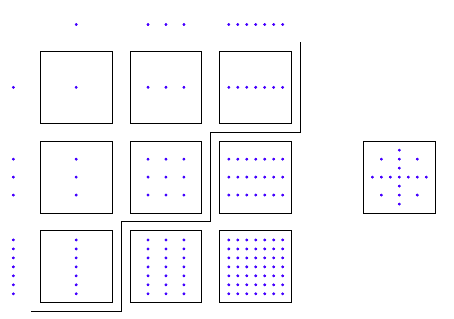
\includegraphics[scale=0.35]{sparse_grids}
        \column{.35\linewidth}
        \caption{Left are product grids $\Delta_{\beta_1} \otimes \Delta_{\beta_2}$ for $1 \le \beta_1, \beta_2 \le 3$. Right is the corresponding SG construction.}
        \label{fig:example right}
      \end{columns}
    \end{figure}
\end{frame}

\begin{frame}[plain,shrink=2]	
	\frametitle{\centerline{ ASGQ in practice }}
	\vspace{0.2cm}
	\begin{itemize}
		\item The construction of \blue{$\mathcal{I}^{\text{ASGQ}}$} is done by \red{profit thresholding}
 \begin{equation*}
 \blue{\mathcal{I}^{\text{ASGQ}}}=\{\boldsymbol{\beta} \in \mathbb{N}^d_{+}: \blue{P_{\boldsymbol{\beta}}}	 \ge \overline{T}\}.
 \end{equation*}
 \item \textbf{Profit of a hierarchical surplus} \blue{$P_{\boldsymbol{\beta}}= \frac{\abs{\Delta E_{\boldsymbol{\beta}}}}{\Delta\mathcal{W}_{\boldsymbol{\beta}}}$}.
\item \textbf{Error contribution}:  \blue{ $\Delta E_{\boldsymbol{\beta}} = \abs{\mathcal{M}^{\mathcal{I} \cup \{\boldsymbol{\beta}\}}-\mathcal{M}^{\mathcal{I}}}$}.
%how much the error decreases if the operator $\Delta[F_{\boldsymbol{\beta}}]$ is added to \blue{$\mathcal{M}_{\mathcal{I}}[F]$
		\item \textbf{Work contribution}:  \blue{$ 		\Delta \mathcal{W}_{\boldsymbol{\beta}} = \text{Work}[\mathcal{M}^{\mathcal{I} \cup \{\boldsymbol{\beta}\}}]-\text{Work}[\mathcal{M}^{\mathcal{I}}]$}.	
		 \begin{figure}
      \begin{columns}
        \column{.5\linewidth}
        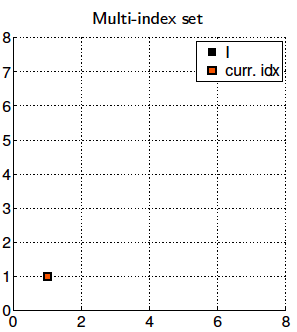
\includegraphics[scale=0.6]{./MISC_construction/1}
        \column{.4\linewidth}
        \caption{\red{A posteriori, adaptive construction} as in \parencite{haji2016multi}: Given an index set $\mathcal{I}_k$, compute the profits of the neighbor indices and select the most profitable one}
        \label{fig:example right}
      \end{columns}
    \end{figure}

		\end{itemize}
		
\end{frame}

\begin{frame}[plain,shrink=2,noframenumbering]	
	\frametitle{\centerline{ ASGQ in practice }}
	\vspace{0.2cm}
	\begin{itemize}
		\item The construction of \blue{$\mathcal{I}^{\text{ASGQ}}$} is done by \red{profit thresholding}
 \begin{equation*}
 \blue{\mathcal{I}^{\text{ASGQ}}}=\{\boldsymbol{\beta} \in \mathbb{N}^d_{+}: \blue{P_{\boldsymbol{\beta}}}	 \ge \overline{T}\}.
 \end{equation*}
 \item \textbf{Profit of a hierarchical surplus} \blue{$P_{\boldsymbol{\beta}}= \frac{\abs{\Delta E_{\boldsymbol{\beta}}}}{\Delta\mathcal{W}_{\boldsymbol{\beta}}}$}.
\item \textbf{Error contribution}:  \blue{ $\Delta E_{\boldsymbol{\beta}} = \abs{\mathcal{M}^{\mathcal{I} \cup \{\boldsymbol{\beta}\}}-\mathcal{M}^{\mathcal{I}}}$}.
%how much the error decreases if the operator $\Delta[F_{\boldsymbol{\beta}}]$ is added to \blue{$\mathcal{M}_{\mathcal{I}}[F]$
		\item \textbf{Work contribution}:  \blue{$ 		\Delta \mathcal{W}_{\boldsymbol{\beta}} = \text{Work}[\mathcal{M}^{\mathcal{I} \cup \{\boldsymbol{\beta}\}}]-\text{Work}[\mathcal{M}^{\mathcal{I}}]$}.	
		 \begin{figure}
      \begin{columns}
        \column{.5\linewidth}
        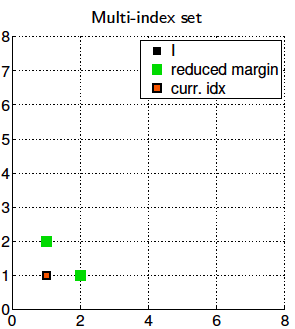
\includegraphics[scale=0.6]{./MISC_construction/2}
        \column{.4\linewidth}
        \caption{\red{A posteriori, adaptive construction} as in \parencite{haji2016multi}: Given an index set $\mathcal{I}_k$, compute the profits of the neighbor indices and select the most profitable one}
        \label{fig:example right}
      \end{columns}
    \end{figure}
			\end{itemize}
\end{frame}

\begin{frame}[plain,shrink=2,noframenumbering]	
	\frametitle{\centerline{ ASGQ in practice }}
	\vspace{0.2cm}
	\begin{itemize}
		\item The construction of \blue{$\mathcal{I}^{\text{ASGQ}}$} is done by \red{profit thresholding}
 \begin{equation*}
 \blue{\mathcal{I}^{\text{ASGQ}}}=\{\boldsymbol{\beta} \in \mathbb{N}^d_{+}: \blue{P_{\boldsymbol{\beta}}}	 \ge \overline{T}\}.
 \end{equation*}
 \item \textbf{Profit of a hierarchical surplus} \blue{$P_{\boldsymbol{\beta}}= \frac{\abs{\Delta E_{\boldsymbol{\beta}}}}{\Delta\mathcal{W}_{\boldsymbol{\beta}}}$}.
\item \textbf{Error contribution}:  \blue{ $\Delta E_{\boldsymbol{\beta}} = \abs{\mathcal{M}^{\mathcal{I} \cup \{\boldsymbol{\beta}\}}-\mathcal{M}^{\mathcal{I}}}$}.
%how much the error decreases if the operator $\Delta[F_{\boldsymbol{\beta}}]$ is added to \blue{$\mathcal{M}_{\mathcal{I}}[F]$
		\item \textbf{Work contribution}:  \blue{$\Delta \mathcal{W}_{\boldsymbol{\beta}} = \text{Work}[\mathcal{M}^{\mathcal{I} \cup \{\boldsymbol{\beta}\}}]-\text{Work}[\mathcal{M}^{\mathcal{I}}]$}.
			 \begin{figure}
      \begin{columns}
        \column{.5\linewidth}
        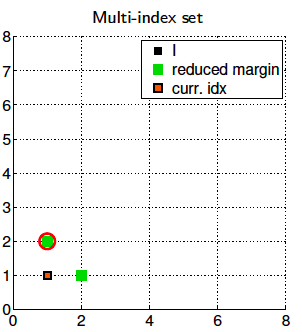
\includegraphics[scale=0.6]{./MISC_construction/3}
        \column{.4\linewidth}
        \caption{\red{A posteriori, adaptive construction} as in \parencite{haji2016multi}: Given an index set $\mathcal{I}_k$, compute the profits of the neighbor indices and select the most profitable one}
        \label{fig:example right}
      \end{columns}
    \end{figure}
	\end{itemize}
\end{frame}
\begin{frame}[plain,shrink=2,noframenumbering]	
	\frametitle{\centerline{ ASGQ in practice }}
	\vspace{0.2cm}
	\begin{itemize}
		\item The construction of \blue{$\mathcal{I}^{\text{ASGQ}}$} is done by \red{profit thresholding}
 \begin{equation*}
 \blue{\mathcal{I}^{\text{ASGQ}}}=\{\boldsymbol{\beta} \in \mathbb{N}^d_{+}: \blue{P_{\boldsymbol{\beta}}}	 \ge \overline{T}\}.
 \end{equation*}
 \item \textbf{Profit of a hierarchical surplus} \blue{$P_{\boldsymbol{\beta}}= \frac{\abs{\Delta E_{\boldsymbol{\beta}}}}{\Delta\mathcal{W}_{\boldsymbol{\beta}}}$}.
\item \textbf{Error contribution}:  \blue{ $\Delta E_{\boldsymbol{\beta}} = \abs{\mathcal{M}^{\mathcal{I} \cup \{\boldsymbol{\beta}\}}-\mathcal{M}^{\mathcal{I}}}$}.
%how much the error decreases if the operator $\Delta[F_{\boldsymbol{\beta}}]$ is added to \blue{$\mathcal{M}_{\mathcal{I}}[F]$
		\item \textbf{Work contribution}:  \blue{$ 		\Delta \mathcal{W}_{\boldsymbol{\beta}} = \text{Work}[\mathcal{M}^{\mathcal{I} \cup \{\boldsymbol{\beta}\}}]-\text{Work}[\mathcal{M}^{\mathcal{I}}]$}.
			 \begin{figure}
      \begin{columns}
        \column{.5\linewidth}
        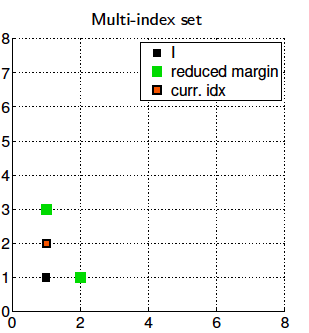
\includegraphics[scale=0.6]{./MISC_construction/4}
        \column{.4\linewidth}
        \caption{\red{A posteriori, adaptive construction} as in \parencite{haji2016multi}: Given an index set $\mathcal{I}_k$, compute the profits of the neighbor indices and select the most profitable one}
        \label{fig:example right}
      \end{columns}
    \end{figure}
	\end{itemize}
\end{frame}

\begin{frame}[plain,shrink=2,noframenumbering]	
	\frametitle{\centerline{ ASGQ in practice }}
	\vspace{0.2cm}
	\begin{itemize}
		\item The construction of \blue{$\mathcal{I}^{\text{ASGQ}}$} is done by \red{profit thresholding}
 \begin{equation*}
 \blue{\mathcal{I}^{\text{ASGQ}}}=\{\boldsymbol{\beta} \in \mathbb{N}^d_{+}: \blue{P_{\boldsymbol{\beta}}}	 \ge \overline{T}\}.
 \end{equation*}
 \item \textbf{Profit of a hierarchical surplus} \blue{$P_{\boldsymbol{\beta}}= \frac{\abs{\Delta E_{\boldsymbol{\beta}}}}{\Delta\mathcal{W}_{\boldsymbol{\beta}}}$}.
\item \textbf{Error contribution}:  \blue{ $\Delta E_{\boldsymbol{\beta}} = \abs{\mathcal{M}^{\mathcal{I} \cup \{\boldsymbol{\beta}\}}-\mathcal{M}^{\mathcal{I}}}$}.
%how much the error decreases if the operator $\Delta[F_{\boldsymbol{\beta}}]$ is added to \blue{$\mathcal{M}_{\mathcal{I}}[F]$
		\item \textbf{Work contribution}:  \blue{$ 		\Delta \mathcal{W}_{\boldsymbol{\beta}} = \text{Work}[\mathcal{M}^{\mathcal{I} \cup \{\boldsymbol{\beta}\}}]-\text{Work}[\mathcal{M}^{\mathcal{I}}]$}.
			 \begin{figure}
      \begin{columns}
        \column{.5\linewidth}
        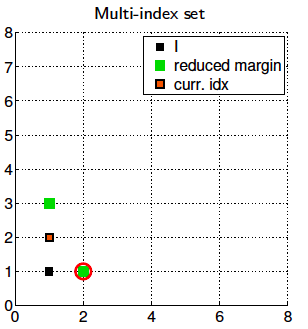
\includegraphics[scale=0.6]{./MISC_construction/5}
        \column{.4\linewidth}
        \caption{\red{A posteriori, adaptive construction} as in \parencite{haji2016multi}: Given an index set $\mathcal{I}_k$, compute the profits of the neighbor indices and select the most profitable one}
        \label{fig:example right}
      \end{columns}
    \end{figure}
			
	\end{itemize}
\end{frame}

\begin{frame}[plain,shrink=2,noframenumbering]	
	\frametitle{\centerline{ ASGQ in practice }}
	\vspace{0.2cm}
	\begin{itemize}
		\item The construction of \blue{$\mathcal{I}^{\text{ASGQ}}$} is done by \red{profit thresholding}
 \begin{equation*}
 \blue{\mathcal{I}^{\text{ASGQ}}}=\{\boldsymbol{\beta} \in \mathbb{N}^d_{+}: \blue{P_{\boldsymbol{\beta}}}	 \ge \overline{T}\}.
 \end{equation*}
 \item \textbf{Profit of a hierarchical surplus} \blue{$P_{\boldsymbol{\beta}}= \frac{\abs{\Delta E_{\boldsymbol{\beta}}}}{\Delta\mathcal{W}_{\boldsymbol{\beta}}}$}.
\item \textbf{Error contribution}:  \blue{ $\Delta E_{\boldsymbol{\beta}} = \abs{\mathcal{M}^{\mathcal{I} \cup \{\boldsymbol{\beta}\}}-\mathcal{M}^{\mathcal{I}}}$}.
%how much the error decreases if the operator $\Delta[F_{\boldsymbol{\beta}}]$ is added to \blue{$\mathcal{M}_{\mathcal{I}}[F]$
		\item \textbf{Work contribution}:  \blue{$ 		\Delta \mathcal{W}_{\boldsymbol{\beta}} = \text{Work}[\mathcal{M}^{\mathcal{I} \cup \{\boldsymbol{\beta}\}}]-\text{Work}[\mathcal{M}^{\mathcal{I}}]$}.	
		 \begin{figure}
      \begin{columns}
        \column{.5\linewidth}
        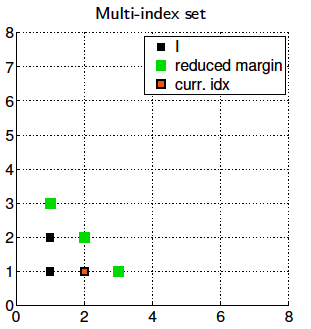
\includegraphics[scale=0.6]{./MISC_construction/6}
        \column{.4\linewidth}
        \caption{\red{A posteriori, adaptive construction} as in \parencite{haji2016multi}: Given an index set $\mathcal{I}_k$, compute the profits of the neighbor indices and select the most profitable one}
        \label{fig:example right}
      \end{columns}
    \end{figure}

	
	\end{itemize}
\end{frame}

%\begin{frame}[plain,shrink=2,noframenumbering]	
%	\frametitle{\centerline{ ASGQ in practice }}
%	\vspace{0.2cm}
%	\begin{itemize}
%		\item The construction of \blue{$\mathcal{I}^{\text{ASGQ}}$} is done by \red{profit thresholding}
% \begin{equation*}
% \blue{\mathcal{I}^{\text{ASGQ}}}=\{\boldsymbol{\beta} \in \mathbb{N}^d_{+}: \blue{P_{\boldsymbol{\beta}}}	 \ge \overline{T}\}.
% \end{equation*}
% \item \textbf{Profit of a hierarchical surplus} \blue{$P_{\boldsymbol{\beta}}= \frac{\abs{\Delta E_{\boldsymbol{\beta}}}}{\Delta\mathcal{W}_{\boldsymbol{\beta}}}$}.
%\item \textbf{Error contribution}:  \blue{ $\Delta E_{\boldsymbol{\beta}} = \abs{\mathcal{M}^{\mathcal{I} \cup \{\boldsymbol{\beta}\}}-\mathcal{M}^{\mathcal{I}}}$}.
%%how much the error decreases if the operator $\Delta[F_{\boldsymbol{\beta}}]$ is added to \blue{$\mathcal{M}_{\mathcal{I}}[F]$
%		\item \textbf{Work contribution}:  \blue{$ 		\Delta \mathcal{W}_{\boldsymbol{\beta}} = \text{Work}[\mathcal{M}^{\mathcal{I} \cup \{\boldsymbol{\beta}\}}]-\text{Work}[\mathcal{M}^{\mathcal{I}}]$}.	
%			 \begin{figure}
%      \begin{columns}
%        \column{.5\linewidth}
%        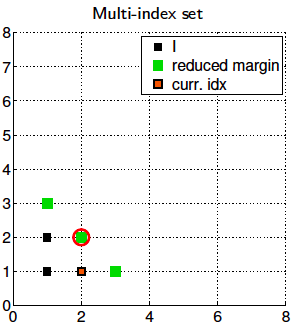
\includegraphics[scale=0.6]{./MISC_construction/7}
%        \column{.4\linewidth}
%        \caption{\red{A posteriori, adaptive construction} as in \cite{haji2016multi}: Given an index set $\mathcal{I}_k$, compute the profits of the neighbor indices and select the most profitable one}
%        \label{fig:example right}
%      \end{columns}
%    \end{figure}
%	\end{itemize}
%\end{frame}


\begin{frame}[plain, shrink=4]\frametitle{\centerline{Randomized QMC} }  
\begin{itemize}

\item \red{A (rank-$1$) lattice rule} \parencite{sloan1985lattice,nuyens2014construction} with $n$ points 
\begin{equation*}
Q_n(f):=\frac{1}{n}\sum_{k=0}^{n-1} f \left( \frac{kz \: \text{mod}\: n}{n}\right),
\end{equation*}
where  $z = (z_1,\dots, z_d) \in \nset^d$.

\item \red{A randomly shifted lattice rule} 
\begin{align}
\overline{Q}_{n,q}(f)=\frac{1}{q} \sum_{i=0}^{q-1}Q^{(i )}_n(f)=\frac{1}{q}\sum_{i=0}^{q-1}\left(\frac{1}{n}\sum_{k=0}^{n-1} f \left( \frac{kz+\Delta^{(i)}  \: \text{mod}\: n}{n}\right)  \right),
\end{align}
where $\{\Delta^{(i)}\}_{i=1}^q$: independent random shifts, and $M^{\text{QMC}}=q \times n$.

\begin{itemize}
\item  Unbiased approximation of the integral.
\item  Practical error estimate.
\end{itemize}
%\item We use a pre-made point generators using latticeseq\_b2.py from   \url{https://people.cs.kuleuven.be/~dirk.nuyens/qmc-generators/}.
\end{itemize}

\end{frame}



\begin{frame}[plain,shrink=8]\frametitle{\centerline{Wiener path generation methods} }  
$\{t_i\}_{i=0}^{N}$: Grid of time steps, $\{B_{t_i}\}_{i=0}^{N}$: Brownian motion increments 
		\begin{itemize}
			\item \textbf{\red{Random Walk}}
			\begin{itemize}
				\item Proceeds incrementally, given $B_{t_i}$,
					\begin{equation*}
				B_{t_{i+1}}=B_{t_i}+ \sqrt{\Delta t} z_i, \: z_i \sim \mathcal{N}(0,1) \PERIOD
				\end{equation*}
				\item All components of $\mathbf{z} = (z_1,\dots,z_N)$ have the same scale of importance: \red{isotropic}.
			\end{itemize}
			\item \textbf{\red{Hierarchical Brownian Bridge}} 
			\begin{itemize}
				\item Given a past value $B_{t_i}$ and a future value $B_{t_k}$, the value $B_{t_j}$ (with $t_i < t_j < t_k$) can be generated according to ($\rho=\frac{j-i}{k-i}$)
				\begin{equation*}\label{eq: Brownian Bridge construction}
				B_{t_j}=(1-\rho) B_{t_i}+\rho B_{t_k}+ \sqrt{\rho (1-\rho)(k-i) \Delta t} z_j, \: z_j \sim \mathcal{N}(0,1) \PERIOD
				\end{equation*}
					\item The most important values (determine the large scale structure of Brownian motion) are the first components of $\mathbf{z} = (z_1,\dots,z_N)$.
					\item $\searrow$ the \red{effective dimension} ($\#$ important dimensions) by $\nearrow$  \red{anisotropy} between different directions $\Rightarrow$ \red{Faster} ASGQ and QMC convergence.
			\end{itemize} 
		
	\end{itemize}
\end{frame}



\begin{frame}[plain, shrink=10]\frametitle{\centerline{Richardson Extrapolation \parencite{talay1990expansion}}}
\vspace{0.2cm}

\textbf{\blue{Motivation}}
\begin{itemize}
\item $(X_t)_{0 \le t \le T}$ a certain stochastic process,  $(\widehat{X}_{t_i}^h)_{0 \le  t_i \le T}$ its approximation using a suitable  scheme with a time step $h$. 
\item For sufficiently small $h$, and a suitable smooth function $f$, assume 
\begin{align*}
	\expt{f(\widehat{X}_T^h)}= \expt{f(X_T)} + c h +\Ordo{h^2} \PERIOD
\end{align*}
$$\Rightarrow 2 \expt{f(\widehat{X}_T^{2h})}- \expt{f(\widehat{X}_T^{h})} =\expt{f(X_T)} + \Ordo{h^2} .$$
\end{itemize} 
\textbf{\blue{General Formulation}}

 $\{h_J=h_0 2^{-J}\}_{J\ge 0}$:  \red{grid sizes}, $K_\text{R}$:  \red{level of  Richardson extrapolation}, $I(J,K_\text{R})$: \red{approximation of $\expt{f(X_T)}$ by terms up to level $K_\text{R}$} 
\begin{small}
\begin{align}
I(J,K_\text{R})=\frac{2^{K_\text{R}}I(J,K_\text{R}-1)-I(J-1,K_\text{R}-1)}{2^{K_\text{R}}-1},\quad J=1,2,\dots, K_\text{R}=1,2,\dots
\end{align}
\end{small}
\textbf{\blue{Advantage}}

Applying level $K_\text{R}$ of Richardson extrapolation  \red{dramatically reduces the bias} $\Rightarrow \searrow$ \red{the  number of time steps $N$ needed}  to achieve a certain error tolerance $\Rightarrow \searrow$  \red{the total dimension} of the integration problem.
\end{frame}



\section{Numerical Experiments and Results}
\frame[plain,noframenumbering]{\tableofcontents[currentsection,currentsubsection]}



\begin{frame}[plain,shrink=8]\frametitle{\centerline{Numerical experiments}}
\vspace{0.3cm}
\begin{table}[!h]
\begin{small}
	\centering
\caption{Reference solution (\red{using MC with $500$ time steps and number of samples, $M=8 \times 10^6$}) of call option price under the rough Bergomi model, for different parameter constellations.  The numbers between parentheses correspond to the statistical errors estimates.}
\label{table:Reference solution, using MC with $500$ time steps, of Call option price under rBergomi model, for different parameter constellation.}
	\begin{tabular}{l*{2}{c}r}
	\toprule[1.5pt]
		\textbf{Parameters}            & \textbf{Reference solution}    \\
	\hline
		
			$H=0.07, K=1,S_0=1, T=1, \rho=-0.9, \eta=1.9,\xi_0=  0.0552$   & $\underset{(5.6e-05)}{0.0791}$  \\	
		
		$H=0.02, K=1, S_0=1, T=1,\rho=-0.7, \eta=0.4,\xi_0=0.1$   & $\underset{(9.0e-05)}{0.1246}$  \\
		$H=0.02, K=0.8,S_0=1,T=1, \rho=-0.7, \eta=0.4,\xi_0=0.1$   & $\underset{(5.4e-05)}{0.2412}$  \\
		$H=0.02, K=1.2,S_0=1,T=1, \rho=-0.7, \eta=0.4,\xi_0=0.1$   & $\underset{(8.0e-05)}{0.0570}$  \\
	\bottomrule[1.25pt]
	\end{tabular}
	\end{small}
\end{table}

\begin{itemize}
\item Set $1$ is the  \red{closest to the empirical findings} \parencite{gatheral2018volatility}, suggesting that $\blue{H} \approx 0.1$. The choice $\blue{\nu}= 1.9$ and $\blue{\rho}=-0.9$ is justified by \parencite{bayer2016pricing}.

\item  For the remaining three sets, we test the potential of our method for a \red{very rough case}, where variance reduction methods are inefficient.
\end{itemize}
\end{frame}


\begin{frame}[plain, shrink=2]\frametitle{\centerline{Error comparison}}
\vspace{0.2cm}
$\red{\mathcal{E}_{\text{tot}}}$: the total error of approximating the  expectation in \eqref{BS_formula_rbergomi}.
\begin{itemize}
	\item When using ASGQ estimator, $Q_N$
	\begin{align*}
	\red{\mathcal{E}_{\text{tot}}} & \le \abs{C_{\text{RB}}-C_{\text{RB}}^N}+\abs{C_{\text{RB}}^N-Q_{N}} \le \green{\mathcal{E}_B(N)}+ \blue{\mathcal{E}_Q(\text{TOL}_{\text{ASGQ}},N)},
	\end{align*}
where  $\mathcal{E}_Q$ is the quadrature error, $\green{\mathcal{E}_B}$  is the bias, $\blue{\text{TOL}_{\text{ASGQ}}}$ is a user selected tolerance for ASGQ method.
\item When using randomized QMC or MC estimator,   $Q^{\text{MC (QMC)}}_N$
		\begin{align*}
	\red{\mathcal{E}_{\text{tot}}} & \le \abs{C_{\text{RB}}-C_{\text{RB}}^N}+\abs{C_{\text{RB}}^N-Q^{\text{MC (QMC)}}_N} \le \green{\mathcal{E}_B(N)}+ \blue{\mathcal{E}_{S}(M,N)},
	\end{align*}
	where  $\blue{\mathcal{E}_S}$ is the statistical error, $\blue{M}$ is the number of samples used for MC or randomized QMC method.
	\item $\blue{M^{\text{QMC}}}$ and $\blue{M^{\text{MC}}}$, are chosen so that $\blue{\mathcal{E}_{S,\text{QMC}}(M^{\text{QMC}})}$ and  \blue{$\mathcal{E}_{S,\text{MC}}(M^{\text{MC}})$} satisfy
	\begin{align*}
	\blue{\mathcal{E}_{S,\text{QMC}}(M^{\text{QMC}})}=\blue{\mathcal{E}_{S,\text{MC}}(M^{\text{MC}})}= \green{\mathcal{E}_B(N)}=\frac{\red{\mathcal{E}_{\text{tot}}}}{2}\PERIOD
	\end{align*}
\end{itemize}
\end{frame}

\begin{frame}[plain]\frametitle{\centerline{Relative errors and computational gains}}
\begin{table}[!h]
	\centering
	\caption{ In this table, we highlight the computational gains achieved by ASGQ and QMC over MC method to meet a certain error tolerance. We note that the ratios are computed \red{for the best configuration with Richardson extrapolation for each method}. The ratios $\left(\text{ASGQ}/ \text{MC} \right)$ and $\left(\text{QMC}/ \text{MC} \right)$ are referred to  \red{CPU time ratios}.}
		\begin{tabular}{l*{4}{c}r}
			\toprule[1.5pt]
			\textbf{Parameters}              &  \textbf{Relative error}  & \textbf{ $\left(\text{ASGQ}/ \text{MC} \right)$} & \textbf{$\left(\text{QMC}/ \text{MC} \right)$}\\
			\hline
			Set $1$  &  $1\%$&  $ 7\%$ &  $10\%$\\	
			
			\hline
		Set $2$    &  $0.2\%$&  $5\%$ &  $1\%$\\		
			\hline
		Set $3$   &  $0.4\%$&  $4\%$ &  $5\%$\\	
			\hline
		Set $4$ &  $2\%$&  $20\%$ &  $10\%$\\	
			\bottomrule[1.25pt]
		\end{tabular}
	\label{table:Summary of our numerical results.}
\end{table}
\end{frame}

\begin{frame}[plain]\frametitle{\centerline{Computational work of the MC method}
\centerline{with different configurations }}
\begin{figure}
		\centering
		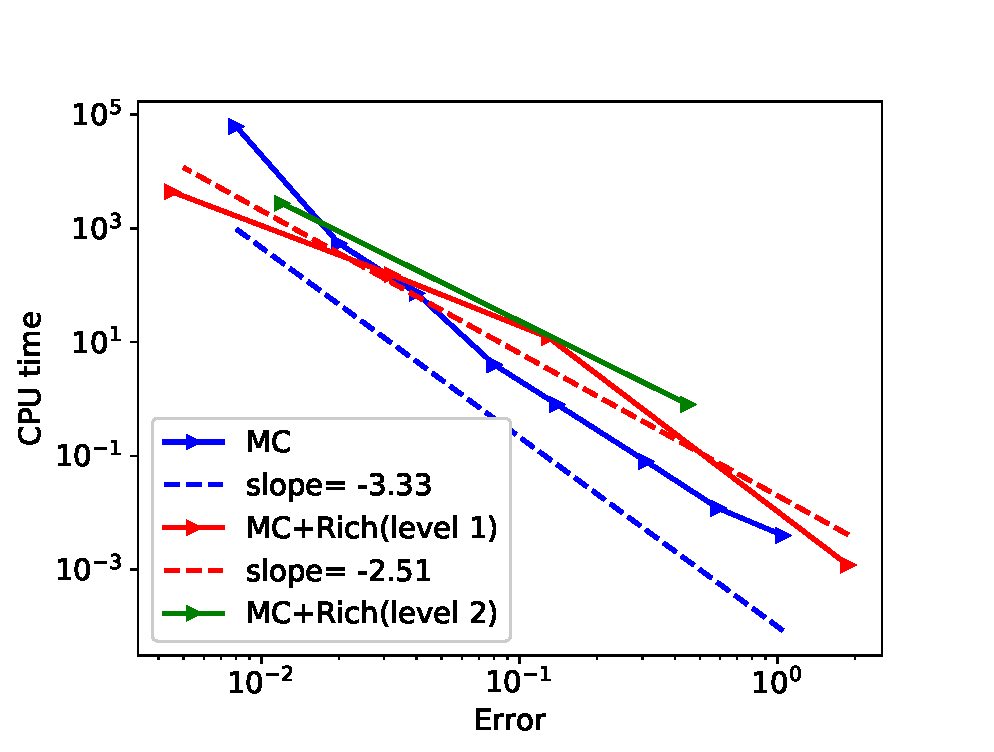
\includegraphics[width=0.7\textwidth]{./rBergomi_Complexity_rates/set2/error_vs_time_set2_MC_comparison}
	\caption{Computational work of the MC  method with the different configurations in terms of  Richardson extrapolation 's level.  Case of \red{parameter set $1$ in Table \ref{table:Reference solution, using MC with $500$ time steps, of Call option price under rBergomi model, for different parameter constellation.}}. }
	\label{fig: Comparing the numerical complexity of the MC  method with the different configurations}
\end{figure}
\end{frame}


\begin{frame}[plain]\frametitle{\centerline{Computational work of the QMC method}
\centerline{with different configurations }}
\begin{figure}
		\centering
		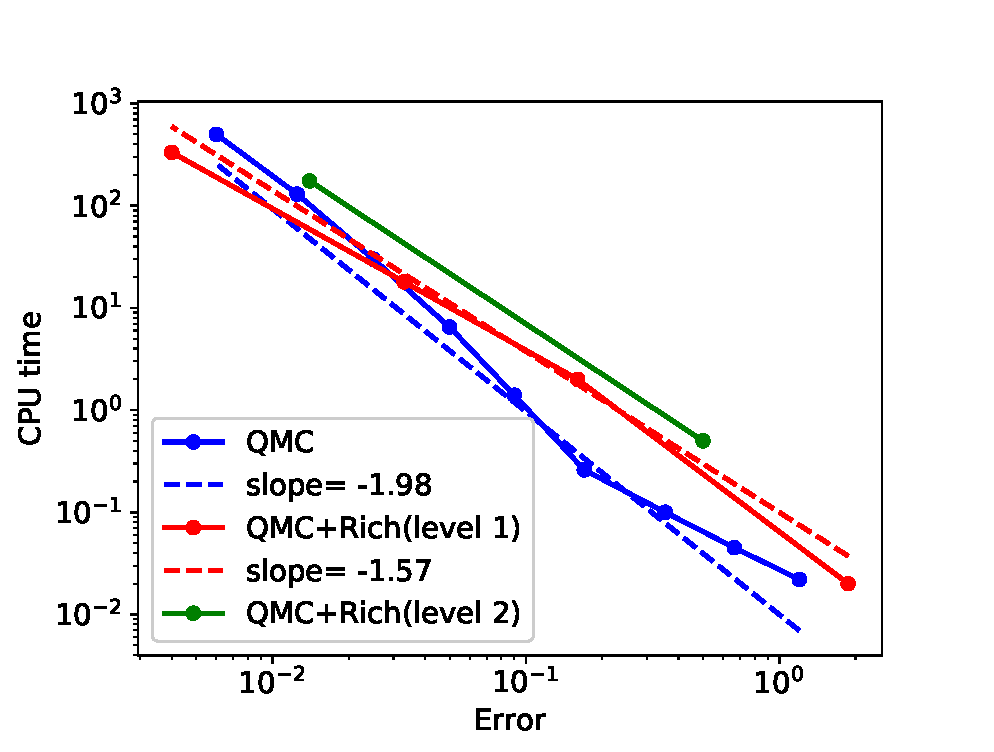
\includegraphics[width=0.7\textwidth]{./rBergomi_Complexity_rates/set2/error_vs_time_set2_QMC_comparison}
	\caption{Computational work of the QMC  method with the different configurations in terms of  Richardson extrapolation 's level.  Case of \red{parameter set $1$ in Table \ref{table:Reference solution, using MC with $500$ time steps, of Call option price under rBergomi model, for different parameter constellation.}}. }
	\label{fig: Comparing the numerical complexity of the QMC  method with the different configurations}
\end{figure}
\end{frame}


\begin{frame}[plain]\frametitle{\centerline{Computational work of the ASGQ method}
\centerline{with different configurations }}
\begin{figure}
		\centering
		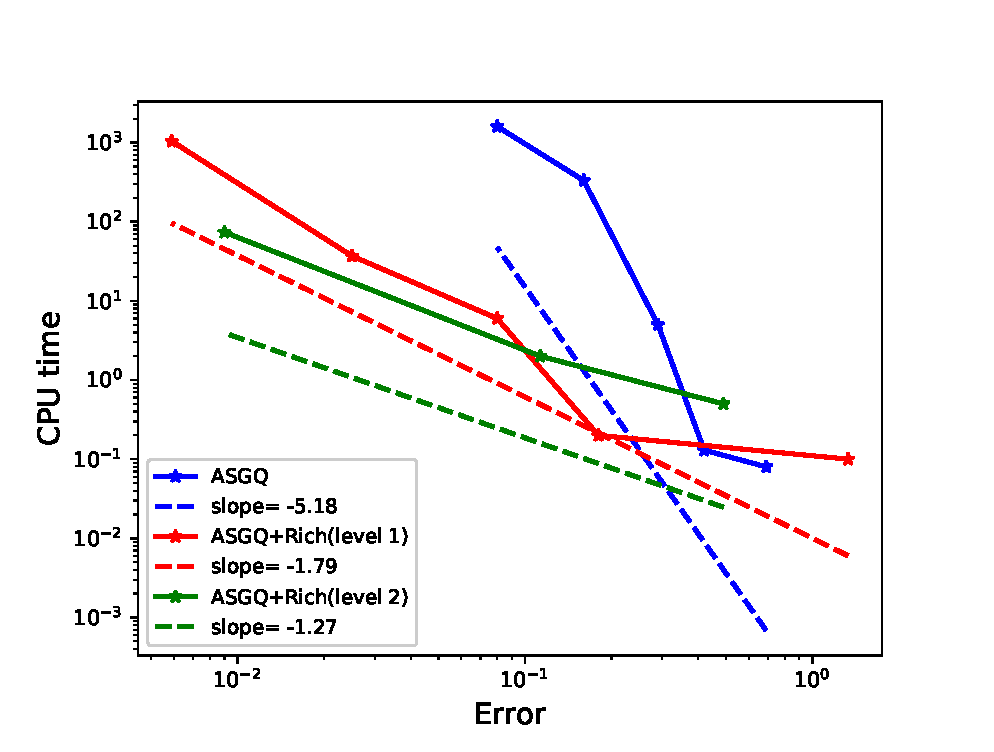
\includegraphics[width=0.7\textwidth]{./rBergomi_Complexity_rates/set2/error_vs_time_set2_MISC_comparison}
	\caption{Computational work of the ASGQ  method with the different configurations in terms of  Richardson extrapolation 's level.  Case of \red{parameter set $1$ in Table \ref{table:Reference solution, using MC with $500$ time steps, of Call option price under rBergomi model, for different parameter constellation.}}. }
	\label{fig: Comparing the numerical complexity of the ASGQ  method with the different configurations}
\end{figure}
\end{frame}


\begin{frame}[plain]\frametitle{\centerline{Computational work of the different methods}
\centerline{with their best configurations}}
\begin{figure}
		\centering
		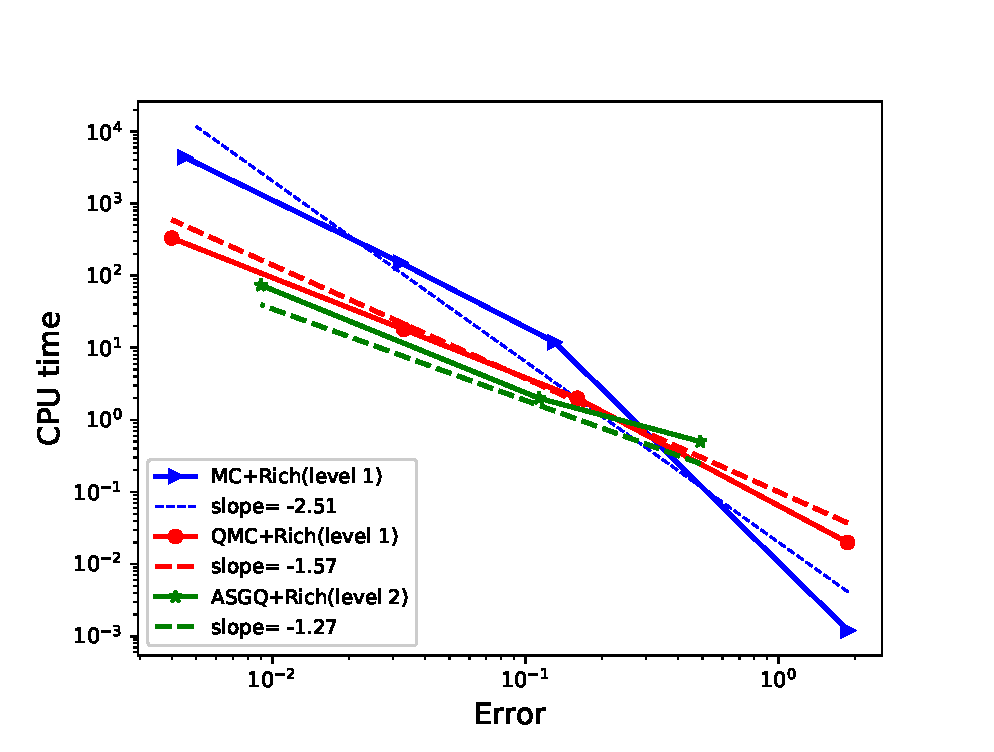
\includegraphics[width=0.72\linewidth]{./rBergomi_Complexity_rates/set2/error_vs_time_set2_full_comparison}
	\caption{Computational work comparison of the different methods \red{with the best configurations}, for the case of \red{parameter set $1$ in Table \ref{table:Reference solution, using MC with $500$ time steps, of Call option price under rBergomi model, for different parameter constellation.}}.}
\label{fig:Complexity plot for  MISC for Case set $2$ parameters, comparison}
\end{figure}
\end{frame}




%%%%%%%%%%%%%%%%%%%%%%%%%%%%%%%%%%%%%%%%%%%%%%%%%%%%%%%%%%%%%%%%%%%%%%%%%%%%%%%%%%%%%%%%%%%%%%%%%%%%%%%%%%%%%%%%%%%%%%%%%%%%
\section{Conclusions}
\frame[plain,noframenumbering]{\tableofcontents[currentsection,currentsubsection]}

\begin{frame}[plain]\frametitle{\centerline{Conclusions}}
\begin{itemize}
\item Proposed  novel \red{fast option pricers}, for options whose underlyings follow \red{the rough Bergomi model}, based on

\begin{itemize}
\item  Conditional expectations for \red{numerical smoothing}. 
\item  \red{Hierarchical deterministic quadrature methods}.
\end{itemize}

\item Given a sufficiently small relative error tolerance, our proposed methods demonstrate \red{substantial computational gains over the standard MC method}, for different parameter constellations.

$\Rightarrow$  \red{Huge cost reduction} when \red{calibrating} under the rough Bergomi model.
\item Accelerating our novel methods can be achieved by using better QMC or ASGQ methods.
%\item More details can be found in  \citefull{bayer2018hierarchical}.

\item More details can be found in 

\fullcite{bayer2018hierarchical}.
\end{itemize}
\end{frame}

%%%%%%%%%%%%%%%%%%%%%%%%%%%%%%%%%%%%%%%%%%%%%%%%%%%%%%%%%%%%%%%%%%%%%%%%%%%%%%%%%%%%%%%%%%%%%%%%%%%%%%%%%%%%%%%%%%%%%%%%%%%%





%%%%%%%%%%%%%%%%%%%%%%%%%%%%%%%%%%%%%%%%%%%%%%%%%%%%%%%%%%%%

%\medskip
%\section{References}

%\begin{frame}[plain,allowframebreaks]
%	\frametitle{References}
%%	\raggedright
%%	\nocite{*}
%\small \bibliographystyle{apalike}
%	\bibliography{smoothing_rBergomi}
%\end{frame}

\begin{frame}[plain,allowframebreaks]
	\frametitle{References}
\printbibliography
\end{frame}





%\section*{}
\begin{frame}[plain,,noframenumbering]
	\LARGE\begin{center}
		Thank you for your attention
	\end{center}
\end{frame}





\end{document}